\documentclass[11pt,a4paper]{article}

\usepackage[T1]{fontenc}
\usepackage[utf8]{inputenc}
\usepackage{fullpage}
\usepackage{hyperref}
\usepackage{pgf}
\usepackage{tikz}
\usetikzlibrary{arrows,automata}

\title{\textbf{Ambiruptor: The Lexical Ambiguation
    Interruptor}\\~\\Project Proposal}
% \author{Boumediene Brikci Sid\\
%         Ievgeniia Oshurko\\
%         Maria Boritchev\\
%         Pierre Ohlmann\\
%         Samir Tendjaoui\\
%         Simon Mauras\\
%         Thi Xuan Vu\\
%         Victor Hublitz}

%\date{22th October 2015}

\begin{document}

\maketitle

\vspace{1cm}
\section*{Presentation}
%Throughout the second year at the ENS Lyon (first year of master), students have to work on an integrated project. This paper describes the proposal of the Ambiruptor project which is born from the merge of the NER project and the Joke Generator project.

The main objective is to produce an efficient tool that gives the correct meaning of an ambiguous text. Our tool will be based on several machine learning concepts. We are going to use annotated texts from the internet to train our tool and resolve ambiguities in texts.

Our team consists of 8 members: Boumediene Brikci Sid, Ievgeniia Oshurko, Maria Boritchev, Pierre Ohlmann, Samir Tendjaoui, Simon Mauras, Thi Xuan Vu and Victor Hublitz. The coordinators of the project are Simon Mauras and Ievgeniia Oshurko.
\vspace{1cm}
\tableofcontents

\newpage

\section*{Motivation}

Word Sense Disambiguation is a Natural Language Processing task that lies in assignment of appropriate meaning of the word according to the given context, and its separation from other possible meanings.
Possible applications of Word Sense Disambiguation:
\begin{itemize}
	\item Machine Translation.
	\item Information Retrieval.
	\item Semantic Parsing.
	\item Speech Synthesis and Recognition.
\end{itemize}

\section{Objectives}

The aim of our project is to develop a tool for disambiguation of text written in natural language. In order to do that we are going to:
\begin{itemize}
	\item Mine data from existing sources.
	\item Preprocess data into training corpus.
	\item Create a tool using learning algorithms.
	\item Evaluate our model.
	\item Create user-friendly interfaces (if we have time).
\end{itemize}

\section{Plan of Our Work}
\subsection{Research on the State of the Art}

The first part of our work is going to be bibliographical search. On this stage we are going to split in 3 groups working on the following topics:
\begin{itemize}
	\item Usual technics for text disambiguation.
	\item Machine learning algorithms.
	\item Existing tools for data mining.
\end{itemize}
The goal of the first topic is to find what has already been done and what is currently studied. The purpose of the second group is to compile a list of several machine learning technics that can be used to solve our problem. The third group is going to look for tools that would enable us to mine workable data from the internet.
At the end of this part, each group is going to do a quick summary on their results, so that everyone is aware of each part.

\subsection{Design}

During the second part we are going to think about the detailed structure and the design of the software we want to implement. 

%\begin{tikzpicture}[->,>=stealth',node distance=4cm]
%  \node[]           (W)             {Wiki};
%  \node[state,rectangle]  (D) [right of=W] {Data};
%  \node[state,rectangle]  (P) [right of=D] {Processing};
%  \node[state,rectangle]  (F) [right of=P] {Features\\extraction};
%\end{tikzpicture}

%The deadline for the end of this part is fixed on \textbf{November the 26th, 2015}.

\subsection{Intermediate report}

%We set the deadline for our intermediate report to \textbf{December the 3rd, 2015}.
The intermediate report will clarify all the details of the upcoming implementation. A small group of two or three people will summarize the decisions made during the design part.

\subsection{Implementation}

The implementation will be divided between 2 groups:
\begin{itemize}
	\item Adaptation of the chosen tools to extract workable data from the internet.
	\item Coding of the different modules (defined during the design part).
\end{itemize}
The progress of the second group depends on the results of the first group.

%The deadline for the end of the implementation part is fixed on \textbf{January the 20th, 2016}.

\subsection{Testing}

We will launch our tool on all the data we are able to process and it might take a while. Validity measures will be estimated.

\subsection{Addons}

As soon as the Ambiruptor tool becomes functional, the creation of user-friendly interfaces will be assigned to a small group of students.
\begin{itemize}
	\item Web application.
	\item Pdf reader plugin.
\end{itemize}
We can expand this part if the project goes well and fast, as we can shorten it if we get stuck in one of the previous parts.

%The deadline for implementation, testing and addons is fixed on \textbf{March the 23th, 2016}.

\subsection{Final report}

%The final report's deadline is fixed on \textbf{April the 15th, 2016} (one month before the public presentation).
All students will summarize their year's work. Two or three people will compile those documents and write the final report.

\section{Organization}

\subsection{Project Management}

\begin{itemize}
	\item Git repository: \url{https://github.com/Ambiruptor}
	\item Mailing list: \href{mailto:ambiruptor@ens-lyon.fr}{\texttt{ambiruptor@ens-lyon.fr}}
\end{itemize}

\subsection{Gantt chart}

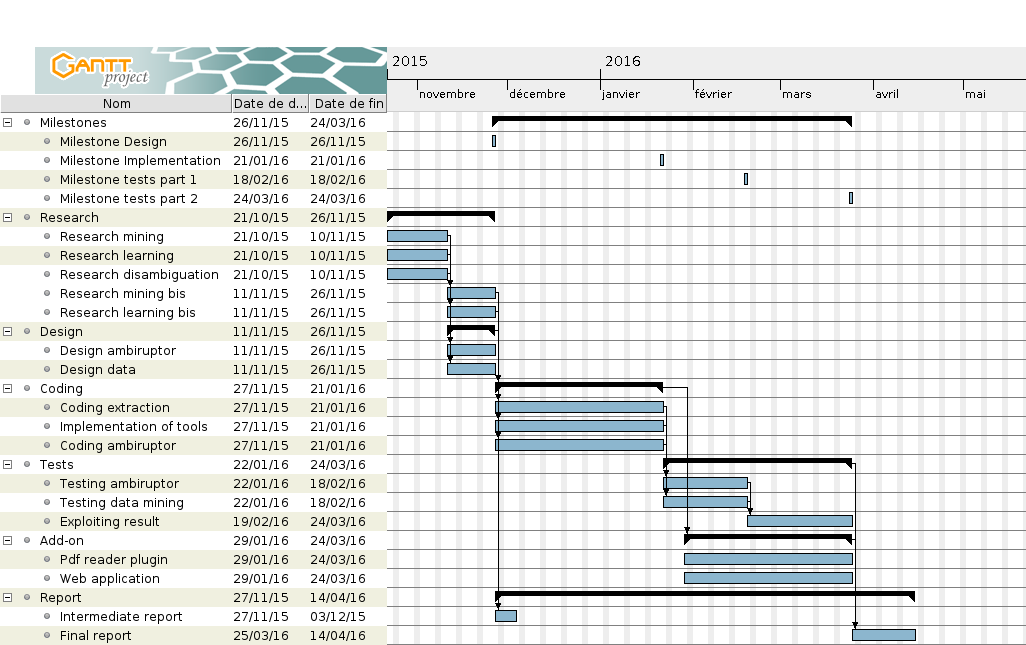
\includegraphics[width=\textwidth]{ambiruptor.png}

\subsection{Milestones}

\begin{itemize}
	\item 26/11/2015 : The architecture of the project is finished.
	\item 03/12/2015 : Deadline for the intermediate report.
	\item 21/01/2015 : The implementation is finished.
	\item 18/02/2015 : First results of the tests.
	\item 24/03/2015 : Tests are completed.
	\item 14/04/2015 : Deadline for the final report.
\end{itemize}

\end{document}